\chapter{Contexte general du projet :}
\section{Presentation du centre :}
Le Code 212 est un centre de formation et de certification dans les metiers du digital, lance dans le cadre du Plan d'Acceleration de la Croissance et de la Transformation de l'economie (PACTE) ESRI-2030 au Maroc. Ce programme vise à repondre aux enjeux actuels et futurs lies à l'emergence des technologies numeriques en offrant des filières specifiques et des formations certifiantes. L'objectif est de renforcer les competences et les qualifications dans le secteur numerique, contribuant ainsi à l'atteinte des objectifs de developpement du pays, notamment celui de faire passer la part du secteur numerique à 5% du PIB d'ici 2035.

Le principal objectif du Centre Code 212 est de former une nouvelle generation de professionnels qualifies dans le domaine du numerique afin de repondre aux besoins croissants du marche de l'emploi dans ce secteur en plein essor. En offrant des formations specialisees et des certifications reconnues, le centre vise à fournir aux apprenants les competences et les connaissances necessaires pour reussir dans des domaines tels que le developpement web, la cybersecurite, l'analyse de donnees, le marketing digital et bien d'autres. En outre, le centre s'engage à promouvoir l'innovation et l'entrepreneuriat en encourageant les initiatives creatives et en offrant un environnement propice à l'emergence de projets novateurs dans le domaine du digital.

\subsection{Fiche du centre Code 212}

\begin{tabularx}{\textwidth}{|l|X|}
\hline
\textbf{Nom du Centre} & Code 212 \\
\hline
\textbf{Domaine d'Activite} & Formation et certification dans les metiers du digital \\
\hline
\textbf{Programme} & Plan d'Acceleration de la Croissance et de la Transformation de l'economie (PACTE) ESRI-2030 \\
\hline
\textbf{Localisation} & Agadir Maroc \\
\hline
\textbf{Objectif} & Renforcer les competences et les qualifications dans le secteur numerique \\
\hline
\textbf{Domaines de Formation} & 
\begin{tabular}{@{}l@{}}
- Developpement web \\
- Cybersecurite \\
- Analyse de donnees \\
- Marketing digital \\
- et bien d'autres
\end{tabular} \\
\hline
\textbf{Engagement} & 
\begin{tabular}{@{}l@{}}
- Promouvoir l'innovation \\
- Encourager l'entrepreneuriat \\
- Offrir un environnement propice aux projets novateurs
\end{tabular} \\
\hline
\end{tabularx}


\subsection{Centre Code212}
\begin{figure}[H]
\centering
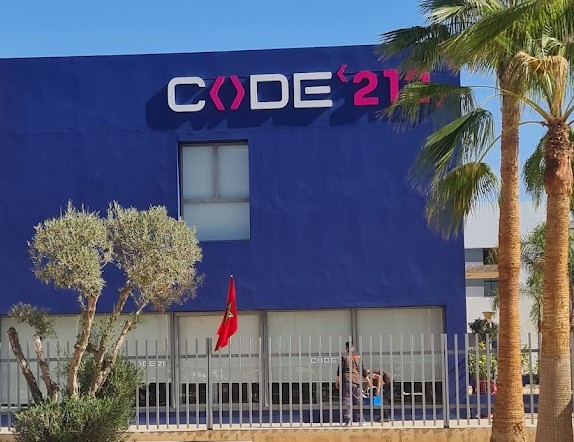
\includegraphics[height=10cm , width=\textwidth]{assets/images/code.jpg}
\caption{Centre Code 212 Agadir}
\label{fig:imagecentre}
\end{figure}

\begin{figure}[H]
\centering
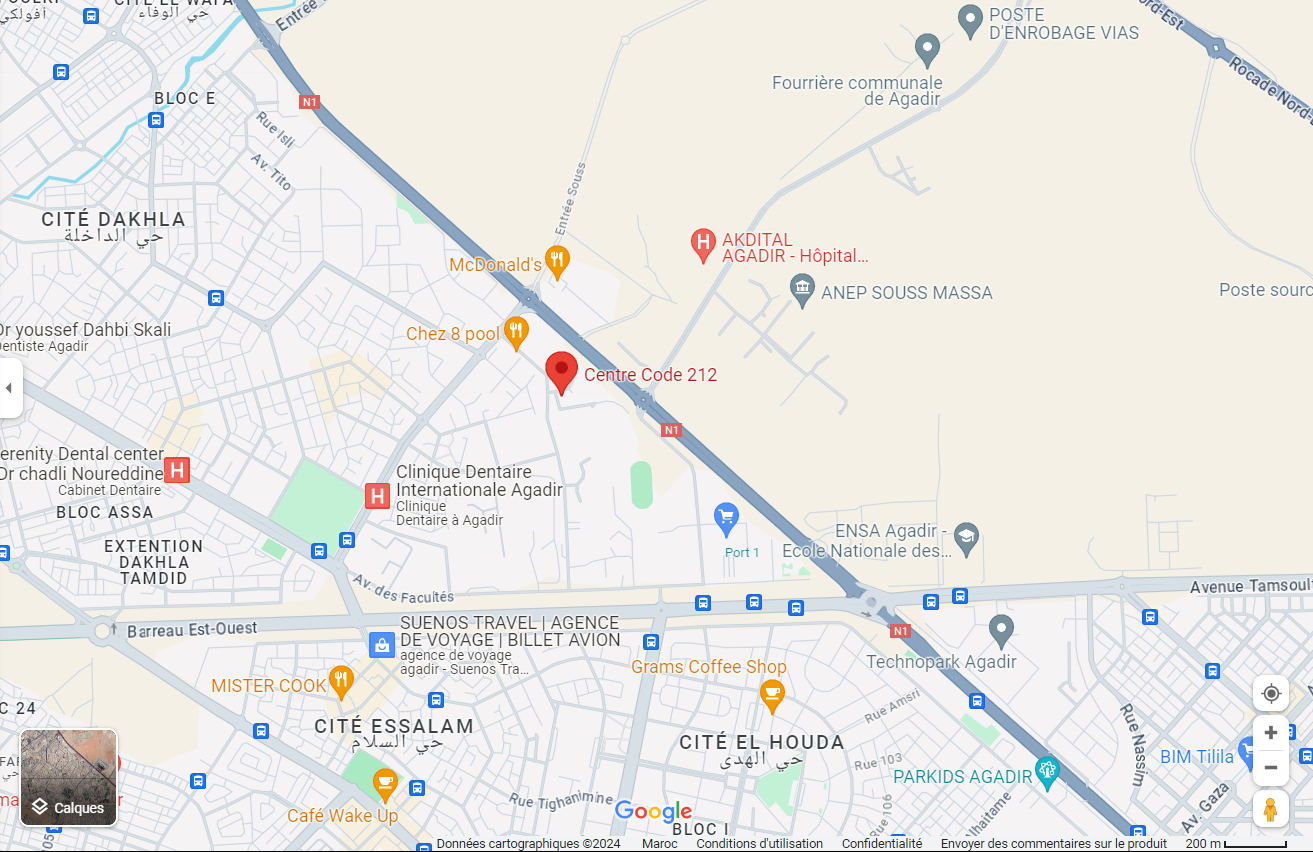
\includegraphics[height=10cm , width=\textwidth]{assets/images/maps.png}
\caption{Localisation du centre}
\label{fig:localisationcentre}
\end{figure}

\subsection{Domaines d'activites et expertise :}

Le centre Code 212 d'Agadir developpe son expertise autour de plusieurs axes strategiques, visant à repondre aux exigences du marche numerique moderne et aux besoins de transformation digitale du Maroc.

\subsubsection{Education et Pedagogie innovante :}

\paragraph{Methodologie d'apprentissage :}
L'education au sein du centre Code 212 repose sur une approche pedagogique revolutionnaire qui rompt avec les methodes traditionnelles d'enseignement. Cette methode, connue sous le nom de \textbf{peer-to-peer learning}, place l'apprenant au centre du processus educatif et favorise :

\begin{itemize}
    \item \textbf{Apprentissage collaboratif} : Les etudiants travaillent en equipes pour resoudre des projets concrets, simulant ainsi l'environnement professionnel reel
    \item \textbf{Autonomie pedagogique} : Absence de cours magistraux traditionnels, encourageant l'auto-apprentissage et la recherche personnelle
    \item \textbf{Mentorat mutuel} : Les etudiants avances accompagnent les debutants, creant une dynamique d'entraide et de partage de connaissances
    \item \textbf{Evaluation par les pairs} : Systeme d'evaluation base sur la correction mutuelle des projets
\end{itemize}

\paragraph{Infrastructure technologique :}
Le centre dispose d'equipements de pointe incluant :
\begin{itemize}
    \item Laboratoires informatiques equipes de stations de travail haute performance
    \item Plateforme d'apprentissage en ligne personnalisee
    \item Environnements de developpement integres (IDE) professionnels
    \item Acces aux technologies cloud et aux outils de developpement modernes
\end{itemize}

\subsubsection{Renforcement des competences et employabilite :}

\paragraph{Programmes de formation specialises :}
Code 212 Agadir propose un curriculum adapte aux exigences du marche du travail numerique, structuré autour de plusieurs piliers :

\begin{enumerate}
    \item \textbf{Socle technique fondamental :}
    \begin{itemize}
        \item Algorithmique et structures de donnees
        \item Programmation orientee objet
        \item Bases de donnees et gestion de l'information
        \item Architectures logicielles et design patterns
    \end{itemize}
    
    \item \textbf{Technologies emergentes :}
    \begin{itemize}
        \item Intelligence artificielle et machine learning
        \item Developpement web full-stack (Frontend/Backend)
        \item Applications mobiles natives et cross-platform
        \item Cloud computing et DevOps
        \item Cybersecurite et protection des donnees
    \end{itemize}
    
    \item \textbf{Competences transversales :}
    \begin{itemize}
        \item Gestion de projets agiles (Scrum, Kanban)
        \item Travail en equipe et communication
        \item Entrepreneuriat et innovation
        \item Veille technologique et apprentissage continu
    \end{itemize}
\end{enumerate}

\paragraph{Partenariats et insertion professionnelle :}
Le centre maintient des relations etroites avec l'ecosysteme economique local et national :
\begin{itemize}
    \item \textbf{Partenariats entreprises} : Collaboration avec des startups et des multinationales pour des projets reels
    \item \textbf{Stages professionnels} : Programme de stages obligatoires en entreprise
    \item \textbf{Job dating} : Organisation regulière d'evenements de recrutement
    \item \textbf{Incubation} : Accompagnement des projets entrepreneuriaux des etudiants
\end{itemize}

\paragraph{Suivi et accompagnement :}
\begin{itemize}
    \item Coaching personnalise pour chaque etudiant
    \item Suivi post-formation pendant 12 mois
    \item Reseau alumni actif
    \item Formation continue et certification professionnelle
\end{itemize}

\section{Presentation du projet :}

\subsection{Contexte général}

À l'ère du numérique, les réseaux sociaux sont devenus des espaces privilégiés d'expression pour les étudiants universitaires. L'Université Ibn Zohr d'Agadir, l'une des institutions d'enseignement supérieur les plus prestigieuses du Maroc, compte des milliers d'étudiants qui s'expriment quotidiennement sur diverses plateformes numériques. Ces expressions spontanées constituent une mine d'informations précieuses sur le ressenti, les préoccupations et les opinions des étudiants concernant leur expérience universitaire.

\subsection{Problématique}

L'analyse manuelle de ces volumes massifs de données textuelles générées par les étudiants sur les réseaux sociaux s'avère impraticable et chronophage. Face à cette réalité, il devient crucial de développer des outils automatisés capables de détecter, analyser et classifier les sentiments exprimés par les étudiants. Cette problématique soulève plusieurs questions fondamentales :

\begin{itemize}
    \item Comment peut-on comprendre automatiquement les émotions et opinions des étudiants exprimées dans leurs publications sur les réseaux sociaux ?
    \item Quels sont les défis techniques liés au traitement du langage naturel dans le contexte marocain multilingue ?
    \item Comment l'intelligence artificielle peut-elle contribuer à améliorer la compréhension des besoins et préoccupations estudiantines ?
\end{itemize}

\subsection{Objectifs de l'étude}

Cette recherche vise à développer un système intelligent d'analyse des sentiments spécifiquement adapté au contexte universitaire marocain. Les objectifs principaux incluent :

\begin{enumerate}
    \item \textbf{Conception d'un système d'analyse automatisée} : Développer une solution technologique capable de traiter et analyser les contenus textuels des étudiants sur les réseaux sociaux
    \item \textbf{Compréhension des sentiments estudiantins} : Identifier et classifier les émotions dominantes exprimées par les étudiants (joie, frustration, satisfaction, inquiétude, etc.)
    \item \textbf{Adaptation au contexte multilingue} : Prendre en compte la diversité linguistique du Maroc (arabe, français, darija) dans l'analyse des sentiments
    \item \textbf{Contribution à l'amélioration de l'expérience universitaire} : Fournir des insights exploitables pour l'amélioration des services et de l'environnement d'apprentissage
\end{enumerate}

\subsection{Questions de recherche}

Cette étude s'articule autour de plusieurs questions de recherche fondamentales :

\begin{itemize}
    \item \textbf{Question principale} : Comment l'intelligence artificielle peut-elle être utilisée efficacement pour analyser les sentiments des étudiants de l'Université Ibn Zohr exprimés sur les réseaux sociaux ?
    \item \textbf{Questions secondaires} :
    \begin{itemize}
        \item Quelles sont les méthodes de traitement automatique du langage naturel les plus adaptées au contexte marocain ?
        \item Comment gérer la complexité linguistique et culturelle dans l'analyse des sentiments ?
        \item Quels modèles d'intelligence artificielle offrent les meilleures performances pour cette tâche spécifique ?
        \item Comment intégrer efficacement les différentes modalités d'expression (texte, émojis, images) ?
    \end{itemize}
\end{itemize}

\subsection{Méthodologie de recherche}

Notre approche méthodologique s'appuie sur une démarche scientifique rigoureuse combinant recherche théorique et développement pratique :

\begin{enumerate}
    \item \textbf{Revue de littérature approfondie} : Analyse critique des travaux existants en analyse de sentiments, avec un focus particulier sur les défis du sarcasme, des émojis et de la multimodalité
    \item \textbf{Collecte et préparation des données} : Constitution d'un corpus représentatif de publications d'étudiants sur les réseaux sociaux
    \item \textbf{Développement du système} : Conception et implémentation d'une architecture technique innovante
    \item \textbf{Évaluation et validation} : Tests de performance et validation des résultats obtenus
    \item \textbf{Analyse et interprétation} : Exploitation des résultats pour générer des insights exploitables
\end{enumerate}

\subsection{Cadre de recherche : Fondements théoriques de l'analyse de sentiment}

\subsubsection{Qu'est-ce que le « sentiment » ?}

En psychologie, le sentiment désigne un état affectif durable et d'une intensité modérée, souvent dirigé vers un objet ou une situation donnée. Il se distingue des réactions émotionnelles brèves par sa stabilité temporelle et sa composante cognitive.

Classiquement, William James (1884) fut l'un des premiers à analyser scientifiquement les émotions : il proposa que les changements corporels (rythme cardiaque, tensions musculaires, etc.) précèdent et produisent le ressenti émotionnel. Autrement dit, pour James, sans ces manifestations physiologiques, l'« émotion » ne serait qu'une perception intellectuelle froide de la situation.

Plus tard, Paul Ekman (années 1970) identifia un ensemble d'émotions de base universelles, caractérisées par des expressions faciales distinctes. Ekman a notamment mis en évidence six émotions fondamentales – joie, tristesse, peur, colère, surprise et dégoût – supposées reconnues à travers toutes les cultures.

\subsubsection{Typologie des sentiments}

Du point de vue psychologique, les états affectifs se caractérisent notamment par leur valence émotionnelle, c'est-à-dire le fait d'être agréables ou désagréables (positifs vs négatifs). Cette dimension de valence est fondamentale : par exemple, la peur et la tristesse sont des affects négatifs, alors que la joie est positive.

Dans le langage courant et en analyse de sentiment automatisée, on utilise souvent une typologie simplifiée en trois catégories :

\begin{itemize}
    \item \textbf{Sentiment positif} : reflète un jugement ou une émotion agréable (satisfaction, enthousiasme)
    \item \textbf{Sentiment négatif} : traduit une évaluation défavorable ou une émotion pénible (mécontentement, colère)
    \item \textbf{Sentiment neutre} : indique l'absence de position affective tranchée ou un état mitigé
\end{itemize}

\subsubsection{Distinction entre sentiment et émotion}

Il est crucial de bien distinguer sentiment et émotion, deux termes souvent confondus :

\paragraph{L'émotion} est un épisode bref (de l'ordre de la seconde ou de la minute) accompagné de changements physiologiques marqués (expressions faciales, réactions neurovégétatives, etc.), survenant en réponse immédiate à un stimulus ou un événement spécifique.

\paragraph{Le sentiment} se présente comme un état affectif plus durable qui peut persister des heures, des jours ou davantage. Il s'agit d'une disposition émotionnelle stable, résultant souvent de la maturation ou de la réinterprétation d'émotions passées.

\subsubsection{L'analyse de sentiment dans le NLP}

En Traitement Automatique du Langage Naturel (NLP), l'analyse de sentiment est définie comme le traitement informatique des opinions, évaluations et attitudes exprimées dans un texte. Plus formellement, Bing Liu propose la définition suivante : « L'analyse de sentiment, également appelée opinion mining, est le domaine d'étude qui analyse les opinions, sentiments, évaluations, appréciations, attitudes et émotions des personnes à l'égard d'entités données (produits, services, organisations, individus, événements, etc.) et de leurs attributs ».

L'objectif final est de permettre à un programme de comprendre automatiquement le ressenti exprimé dans des masses de données textuelles non structurées, là où la lecture humaine serait fastidieuse ou impossible à grande échelle.

\subsubsection{Pourquoi l'analyse de sentiment ?}

Plusieurs enjeux majeurs expliquent l'essor de l'analyse de sentiment :

\begin{itemize}
    \item \textbf{Compréhension des opinions} : Les opinions des individus exercent une influence directe sur leurs comportements
    \item \textbf{Traitement de volumes massifs} : À l'ère du numérique, une quantité sans précédent d'avis s'exprime publiquement sur Internet
    \item \textbf{Prise de décision éclairée} : L'analyse automatique permet de synthétiser ces informations qualitatives pour dégager des tendances exploitables
    \item \textbf{Prédiction comportementale} : Un indicateur agrégé du sentiment public peut être corrélé à des événements socio-économiques
\end{itemize}

\subsubsection{Applications de l'analyse de sentiment}

L'analyse de sentiment trouve aujourd'hui des applications dans de nombreux domaines :

\paragraph{Secteur éducatif :}
\begin{itemize}
    \item Évaluation de la satisfaction des étudiants concernant les cours et services universitaires
    \item Analyse des commentaires sur les plateformes d'apprentissage en ligne
    \item Détection précoce de situations de détresse psychologique chez les étudiants
    \item Amélioration continue des méthodes pédagogiques basée sur les retours étudiants
\end{itemize}

\paragraph{Réseaux sociaux et communication :}
\begin{itemize}
    \item Surveillance de l'e-réputation des institutions
    \item Analyse des tendances d'opinion sur des sujets d'actualité
    \item Détection de phénomènes viraux ou de crises naissantes
    \item Personnalisation des contenus et recommandations
\end{itemize}

\subsubsection{Fonctionnement de l'analyse de sentiment}

L'analyse automatique de sentiment repose sur plusieurs approches complémentaires :

\paragraph{Approches d'apprentissage automatique :}
\begin{itemize}
    \item \textbf{Support Vector Machines (SVM)} : Efficaces pour la classification de texte
    \item \textbf{Naive Bayes} : Algorithme populaire pour l'analyse de sentiment
    \item \textbf{Régression logistique} : Utilisée pour la reconnaissance émotionnelle textuelle
\end{itemize}

\paragraph{Approches d'apprentissage profond :}
\begin{itemize}
    \item \textbf{Réseaux de neurones convolutionnels (CNN)} : Pour l'évaluation de sentiment affinée
    \item \textbf{Long Short-Term Memory (LSTM)} : Efficaces pour capturer les dépendances à long terme
    \item \textbf{Modèles Transformer} : BERT, T5, et GPT pour des représentations contextuelles avancées
\end{itemize}

\paragraph{Défis spécifiques :}
\begin{itemize}
    \item \textbf{Détection du sarcasme} : Identifier les énoncés ironiques qui inversent le sentiment apparent
    \item \textbf{Traitement des émojis} : Intégrer la dimension visuelle et émotionnelle des symboles
    \item \textbf{Analyse multimodale} : Combiner texte, images et autres modalités pour une compréhension globale
    \item \textbf{Multilinguisme} : Adapter les méthodes aux spécificités linguistiques locales
\end{itemize}

\section{Solution Proposée}

Dans le cadre de notre projet de recherche, nous proposons de développer une application innovante de détection et d'analyse de sentiments spécifiquement conçue pour traiter les commentaires publiés sur Hespress, l'un des sites d'actualités les plus influents du Maroc. Cette solution technologique vise à automatiser l'analyse des opinions exprimées par les citoyens marocains dans leurs réactions aux articles d'actualité.

\subsection{Vue d'ensemble de la solution}

Notre application d'analyse de sentiments représente une solution complète et moderne qui combine les dernières avancées en intelligence artificielle avec une architecture logicielle robuste et scalable. Le système est conçu pour :

\begin{itemize}
    \item \textbf{Collecter automatiquement} les commentaires d'Hespress en temps réel
    \item \textbf{Analyser et classifier} les sentiments exprimés (positif, négatif, neutre)
    \item \textbf{Présenter les résultats} via une interface utilisateur intuitive et interactive
    \item \textbf{Fournir des insights} exploitables pour comprendre l'opinion publique marocaine
\end{itemize}

\subsection{Architecture technique de la solution}

L'architecture de notre application suit une approche microservices moderne, garantissant la scalabilité, la maintenabilité et la performance. Elle s'articule autour des composants suivants :

\subsubsection{Couche de présentation - Frontend}

\paragraph{Next.js Framework :}
Pour le développement de l'interface utilisateur, nous avons choisi \textbf{Next.js}, un framework React de nouvelle génération offrant :

\begin{itemize}
    \item \textbf{Rendu hybride} : Support du Server-Side Rendering (SSR) et de la génération statique
    \item \textbf{Performance optimisée} : Code splitting automatique et optimisation des images
    \item \textbf{Expérience développeur} : Hot reloading et TypeScript intégré
    \item \textbf{SEO-friendly} : Métadonnées dynamiques et pré-rendu des pages
\end{itemize}

\paragraph{Fonctionnalités de l'interface :}
\begin{itemize}
    \item Tableau de bord analytique avec visualisations en temps réel
    \item Interface de configuration et de paramétrage
    \item Système de rapports et d'exportation de données
    \item Interface responsive adaptée aux appareils mobiles et desktop
\end{itemize}

\subsubsection{Couche logique métier - Backend}

\paragraph{FastAPI Framework :}
Le backend de l'application est développé avec \textbf{FastAPI}, un framework Python moderne caractérisé par :

\begin{itemize}
    \item \textbf{Performance élevée} : Basé sur Starlette et Pydantic, offrant des performances comparables à Node.js
    \item \textbf{Documentation automatique} : Génération automatique de documentation OpenAPI/Swagger
    \item \textbf{Validation des données} : Validation automatique des types avec Pydantic
    \item \textbf{Support asynchrone} : Gestion native des opérations asynchrones
\end{itemize}

\paragraph{Services métier :}
\begin{itemize}
    \item Service d'analyse de sentiments intégrant le modèle IA
    \item Service de gestion des utilisateurs et des permissions
    \item Service de traitement et de stockage des données
    \item Service de génération de rapports et de statistiques
\end{itemize}

\subsubsection{Système d'authentification et d'autorisation}

\paragraph{Keycloak Identity Provider :}
Pour sécuriser l'application, nous utilisons \textbf{Keycloak}, une solution d'identité et d'accès open-source offrant :

\begin{itemize}
    \item \textbf{Single Sign-On (SSO)} : Authentification unique pour tous les services
    \item \textbf{Gestion des rôles} : Système de permissions granulaire
    \item \textbf{Protocoles standards} : Support OAuth 2.0, OpenID Connect, SAML 2.0
    \item \textbf{Fédération d'identité} : Intégration avec des providers externes (Google, Facebook, etc.)
\end{itemize}

\subsubsection{Collecte de données - Web Scraping}

\paragraph{Selenium WebDriver :}
Pour la collecte automatisée des commentaires d'Hespress, nous employons \textbf{Selenium}, un outil de web scraping offrant :

\begin{itemize}
    \item \textbf{Automation complète} : Simulation d'interactions utilisateur réelles
    \item \textbf{Support multi-navigateurs} : Compatible Chrome, Firefox, Safari, Edge
    \item \textbf{Gestion JavaScript} : Exécution de code JavaScript côté client
    \item \textbf{Collecte robuste} : Gestion des éléments dynamiques et des délais de chargement
\end{itemize}

\paragraph{Processus de collecte :}
\begin{enumerate}
    \item Navigation automatique vers les articles d'Hespress
    \item Extraction des commentaires et métadonnées associées
    \item Nettoyage et normalisation des données textuelles
    \item Stockage structuré dans la base de données
\end{enumerate}

\subsubsection{Modèle d'intelligence artificielle}

\paragraph{cardiffnlp/twitter-xlm-roberta-base-sentiment :}
Le cœur de notre système d'analyse repose sur le modèle pré-entraîné \textbf{cardiffnlp/twitter-xlm-roberta-base-sentiment}, spécifiquement optimisé pour :

\begin{itemize}
    \item \textbf{Analyse multilingue} : Support natif de l'arabe, du français et d'autres langues
    \item \textbf{Textes courts informels} : Entraîné sur des données de réseaux sociaux (Twitter)
    \item \textbf{Performance éprouvée} : Résultats de pointe sur les benchmarks d'analyse de sentiment
    \item \textbf{Facilité d'intégration} : Compatible avec la bibliothèque Hugging Face Transformers
\end{itemize}

\paragraph{Caractéristiques techniques du modèle :}
\begin{itemize}
    \item \textbf{Architecture} : XLM-RoBERTa (Cross-lingual Language Model)
    \item \textbf{Taille} : Base model avec 125M de paramètres
    \item \textbf{Classes de sortie} : Positif, Négatif, Neutre avec scores de confiance
    \item \textbf{Contexte} : Traitement de séquences jusqu'à 512 tokens
\end{itemize}

\subsubsection{Couche de stockage}

\paragraph{PostgreSQL Database :}
Pour le stockage principal des données, nous utilisons \textbf{PostgreSQL}, une base de données relationnelle avancée offrant :

\begin{itemize}
    \item \textbf{Robustesse} : Conformité ACID et haute disponibilité
    \item \textbf{Performance} : Optimisations avancées pour les requêtes complexes
    \item \textbf{Extensibilité} : Support JSON/JSONB pour données semi-structurées
    \item \textbf{Sécurité} : Chiffrement et contrôle d'accès granulaire
\end{itemize}

\paragraph{Redis Cache :}
Pour optimiser les performances, nous intégrons \textbf{Redis} comme système de cache :

\begin{itemize}
    \item \textbf{Cache haute performance} : Stockage en mémoire pour accès ultra-rapide
    \item \textbf{Session management} : Gestion des sessions utilisateur
    \item \textbf{Cache des résultats} : Mise en cache des analyses de sentiment fréquentes
    \item \textbf{Pub/Sub messaging} : Communication temps réel entre services
\end{itemize}

\subsubsection{API Gateway et orchestration}

\paragraph{Spring Cloud Gateway :}
L'orchestration des microservices est assurée par \textbf{Spring Cloud Gateway}, offrant :

\begin{itemize}
    \item \textbf{Routage intelligent} : Distribution des requêtes vers les services appropriés
    \item \textbf{Load balancing} : Répartition de charge automatique
    \item \textbf{Sécurité centralisée} : Application uniforme des politiques de sécurité
    \item \textbf{Monitoring} : Surveillance et métriques des performances
\end{itemize}

\subsection{Workflow de traitement des données}

Le processus d'analyse de sentiment suit un pipeline optimisé :

\begin{enumerate}
    \item \textbf{Collecte} : Selenium extrait les commentaires d'Hespress
    \item \textbf{Préprocessing} : Nettoyage, normalisation et tokenisation du texte
    \item \textbf{Analyse} : Le modèle XLM-RoBERTa classifie les sentiments
    \item \textbf{Post-processing} : Agrégation et calcul de statistiques
    \item \textbf{Stockage} : Sauvegarde des résultats dans PostgreSQL
    \item \textbf{Visualisation} : Présentation via l'interface Next.js
\end{enumerate}

\subsection{Avantages de la solution proposée}

Notre solution présente plusieurs avantages concurrentiels :

\begin{itemize}
    \item \textbf{Scalabilité} : Architecture microservices adaptée à la croissance
    \item \textbf{Performance} : Technologies modernes optimisées pour la vitesse
    \item \textbf{Précision} : Modèle IA spécialisé pour le contexte marocain
    \item \textbf{Sécurité} : Standards industriels avec Keycloak
    \item \textbf{Maintenabilité} : Code structuré et documentation automatique
    \item \textbf{Flexibilité} : Intégration facile avec d'autres systèmes
\end{itemize}

\section{Conduite du Projet}

La conduite efficace du projet de developpement de l'application d'analyse de sentiments est essentielle pour repondre aux exigences specifiques d'analyse des commentaires d'Hespress. Cette section explore en detail les processus de conception, de planification et de developpement qui sous-tendent la creation de l'application.

\subsection{Conception}

La phase de conception constitue l'etape fondatrice du projet, où l'equipe definit les objectifs de l'application, identifie les fonctionnalites cles et elabore l'architecture generale du systeme d'analyse de sentiments. Cette phase necessite une comprehension precise des besoins d'analyse et des caracteristiques specifiques des commentaires d'Hespress.

À ce stade, des etudes de faisabilite technique, des analyses de performance des modeles de NLP et des sessions de definition des exigences avec les parties prenantes sont utilisees pour rassembler les specifications et pour esquisser les premiers prototypes de l'interface utilisateur. Les scenarios d'utilisation et les workflows d'analyse sont methodiquement elabores pour garantir que l'application est à la fois performante et techniquement viable.

\subsection{Planification des Taches}

Une planification detaillee accompagne une conception reussie ; elle s'attaque à la complexite du processus de developpement en decomposant le projet en modules gererables. L'equipe du projet etablit un calendrier de realisation, determinant les dependances entre les composants et en allouant les ressources necessaires.

La methodologie Agile est adoptee, permettant une flexibilite et une reactivite accrues face aux changements de requirements ou aux retours des utilisateurs. La creation de sprints, la priorisation des backlogs et les revues regulières de sprint assurent que le projet reste sur la bonne voie et adapte aux exigences changeantes tout au long de son cycle de vie.

\subsection{Developpement et Integrations}

Durant la phase de developpement, l'equipe met en œuvre la conception de l'application en codant les differentes composantes logicielles. Les developpeurs integrent les technologies choisies : Next.js pour le frontend, FastAPI pour le backend, Keycloak pour l'authentification, et le modele de sentiment analysis.

La construction de l'infrastructure technique, comprenant les serveurs, les bases de donnees et l'integration avec les APIs, est rigoureusement testee pour garantir son bon fonctionnement. Une serie exhaustive de tests—tests unitaires, tests d'integration et tests de performance—est realisee pour s'assurer que le systeme est robuste, evolutif et pret pour le deploiement.

\section{Methodologie Scrum et ses roles}

Scrum est une methodologie agile utilisee principalement dans le developpement de logiciels pour gerer des projets complexes et assurer une livraison continue de produits de haute qualite. Elle repose sur des cycles de developpement iteratifs et incrementaux appeles "sprints", qui durent generalement de deux à quatre semaines. Scrum encourage la collaboration, la flexibilite et l'amelioration continue à travers des revues regulières et des retrospectives.

\subsection{Les roles dans Scrum}

\begin{itemize}
    \item \textbf{Product Owner (PO)} : Le Product Owner est responsable de maximiser la valeur du produit resultant du travail de l'equipe de developpement. Il gère le backlog produit, un document evolutif contenant les exigences et les fonctionnalites du produit, en le priorisant selon la valeur ajoutee pour le client et les parties prenantes.
    
    \item \textbf{Scrum Master} : Le Scrum Master est le facilitateur de l'equipe Scrum. Il s'assure que Scrum est compris et applique correctement, en aidant l'equipe à suivre les pratiques et les principes Scrum. Le Scrum Master elimine les obstacles qui peuvent empêcher l'equipe de progresser et veille à ce que l'equipe fonctionne efficacement.
    
    \item \textbf{Equipe de Developpement} : L'equipe de developpement est composee de professionnels qui travaillent ensemble pour livrer des increments de produit potentiellement livrables à la fin de chaque sprint. L'equipe est auto-organisee et interdisciplinaire, possedant toutes les competences necessaires pour accomplir le travail sans dependre d'autres personnes exterieures à l'equipe.
\end{itemize}

\begin{figure}[H]
\centering
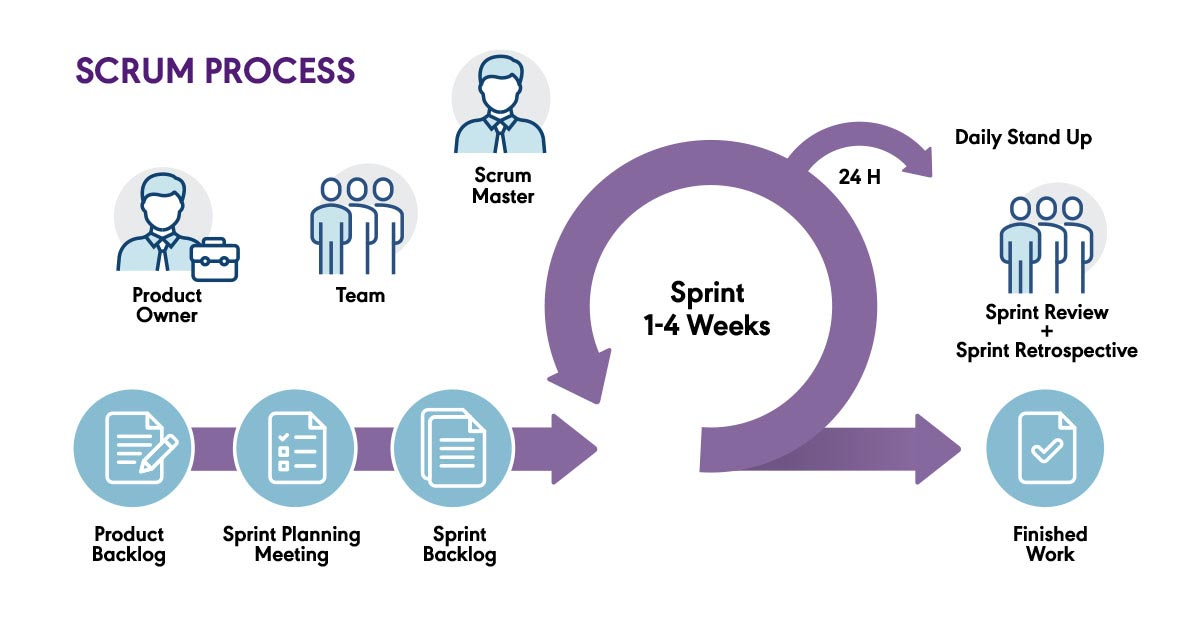
\includegraphics[height=8cm , width=0.8\textwidth]{assets/images/scrum.jpg}
\caption{Methodologie Scrum}
\label{fig:scrum}
\end{figure}

\section{Conclusion}

En conclusion, ce chapitre a mis en lumière la methodologie appliquee dans la conduite du projet de developpement de l'application d'analyse de sentiments pour les commentaires d'Hespress. L'approche methodique de la conception, la rigueur de la planification des taches et l'agilite du developpement ont façonne un outil prometteur pour l'analyse automatisee des opinions publiques.

La maturite du processus adopte reflète notre engagement envers les valeurs d'excellence, de reactivite aux besoins d'analyse et d'innovation constante dans le domaine du traitement automatique du langage naturel.

L'integration entre les technologies de pointe (Next.js, FastAPI, Keycloak, Selenium) et les modeles d'intelligence artificielle avances (XLM-RoBERTa), incarnee par cette application d'analyse de sentiments, est destinee à etablir un nouveau standard en matière d'analyse automatisee des contenus textuels en langue arabe et française.

Avec la fin de ce chapitre, nous anticipons la transition vers les phases subsequentes de mise en œuvre, d'evaluation et d'optimisation, qui seront abordees dans les chapitres suivants. L'impact positif attendu de l'application sur l'analyse des tendances d'opinion et la comprehension des sentiments publics suggère une transformation significative de l'approche d'analyse des donnees textuelles dans le contexte marocain.
